\documentclass{article}
\usepackage{polski}
\usepackage[utf8]{inputenc}
\usepackage{listings}
\usepackage{graphicx}
\graphicspath{ {./image/} }

\author{Tomasz Kowalczyk}
\title{Emulator procesora Zilog Z80}

\begin{document}
	\maketitle
	\tableofcontents
	
	\section{Wstęp}
	\subsection{Cel pracy}
	Celem pracy jest wykonanie \underline{emulatora} procesora Zilog Z80. Aplikacja ta powinna umożliwiać wczytanie programu w postaci kodu maszynowego, deasemblację i wykonanie. Powinny być dostępne dwa tryby wykonania: ciągły i krokowy. W obu przypadkach emulator powinien obrazować stan rejestrów i magistrali wewnętrznych procesora, jak również powinna istnieć możliwość podglądu i zmiany zawartości pamięci programu. Aplikacja powinna być zaimplementowana w języku Java
	
	Z wyżej wymienionych celów, nie zrealizowałem jedynie emulacji wewnętrznych magistrali procesora. Nie posiadając dokumentacji technicznych opisujących wewnętrzną budowę mikroprocesora, jedyną opcją było by poddanie urządzenia inżynierii wstecznej, \underline{co już nie jest tematem tej pracy.}
	
	\subsection{aplikacja}
		
	\begin{figure}[h]
		\caption{Widok główny emulatora}
		\centering
		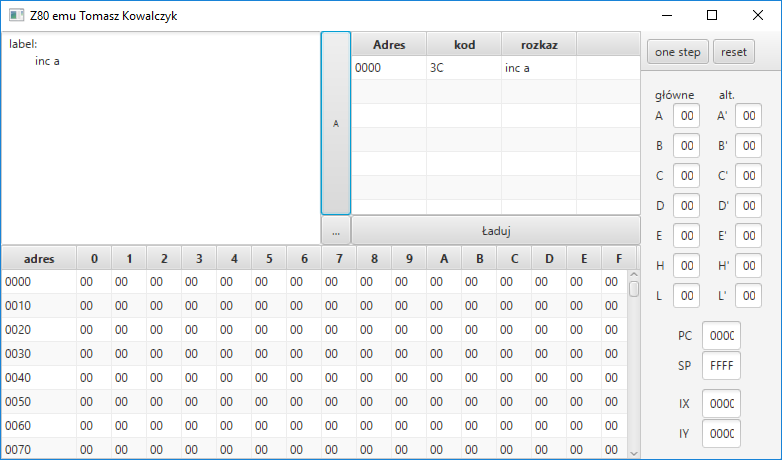
\includegraphics[width=1.0\textwidth]{app1}
	\end{figure}
	
	Interfejs użytkownika podzieliłem na 3 części. 
	\begin{itemize}  
		\item Widok kodu programu napisany w języku asembler, wraz z  wynikowym kodem maszynowym  
		\item Widok pamięci w formie tabeli. Aby uzyskać adres odpowiadający danej komórce, należy dodać do siebie wartość \underline{?????}. Edycje wykonujemy przez dwukrotne kliknięcie na komórce, wpisaniu nowej wartości i zatwierdzeniu klawiszem Enter.
		\item Widok stanu wewnętrznych rejestrów procesora, wraz z przyciskami debugującymi.   
	\end{itemize}
	
	W aplikacji każda wyświetlona wartość jest w systemie heksadecymalnym, i także w takiej notacji wprowadzamy wartości (oprócz pola do edycji kodu asemblera, gdzie możemy używać innych notacji).
	
	\section{Zagadnienie emulacji}
	Treść
	
	\section{Przegląd istniejących rozwiązań}
	Żadne istniejące rozwiązanie nie pozwala na podejrzenie wewnętrznych magistrali procesora
	
	\section{Projekt aplikacji}
	?????
	
	\section{Implementacja}
	Treść
	
	\section{Testy}
		
	\subsection{????}
	Bardzo ważną kwestią w projekcie było dokładne pokrycie kodu aplikacji w testach jednostkowych. Emulator mikro-kontrolera to specyficzna aplikacja, w której nawet mały, wydawałoby się mało znaczący błąd może sprawić że emulator stanie się bezużyteczny. 
	
	Dla przykładu, jeśli dla 3 bajtowego rozkazu procesora zwiększymy rejestr PC o 2 zamiast o 3, to nie wykona się następna instrukcja przewidziana przez programistę. Dalsza praca emulatora stanie się nieprzewidywalna, a następna instrukcja całkowicie “wykolei” nasz program który zacznie wykonywać losowe instrukcje. 
	
	Dlatego poprawne wykonanie każdego rozkazu jest tak ważne dla mojego projektu. Aby uchronić się przed tego typu prostymi błędami każdy emulowany rozkaz posiada swój test/testy jednostkowe napisane przy pomocy biblioteki Junit. 
	
	Przykładowy test dla rozkazu LD A, I. Rozkaz ten ładuje zawartość rejestru A z I:
	\lstinputlisting[language=Java]{listings/exampleTest.java}
	
	Jak widać tak prosta operacja jak skopiowanie wartości z jednego rejestru i przeniesienie go do innego wymaga dosyć objętościowych testów. Oprócz testowania czy poprawna wartość znajduje się rejestrze docelowym musimy sprawdzić także czy flagi CPU zostały ustawione na poprawne wartości, czy ilość przewidywanych cykli zegara została poprawnie zwiększona, czy rejestr PC został zainkrementowany. 
	
	\subsection{Test-driven development}
	TDD to metoda pisania oprogramowania. Zakłada ona że test jednostkowy dla danej funkcjonalności powstaje jako pierwszy. Dopiero po napisaniu testu implementujemy kod programu, a następnie testujemy za pomocą już napisanych testów. Za pomocą TDD była pisana cała aplikacja
	
	\section{Uwagi i wnioski}
	Treść
	
\end{document}